
\documentclass[11pt, twoside]{report}
%% Packages to be used %%
\usepackage{amsmath,amsfonts,amsthm}
\usepackage[a4paper, top=30mm, bottom=25mm, right=30mm, left=25mm]{geometry}
% \usepackage{qcircuit}
\usepackage{fontenc}
\usepackage{graphicx}
\usepackage[english]{babel}
\usepackage{lipsum}
\usepackage{xcolor}
\usepackage{titling}
% \usepackage{cite}
\usepackage[most]{tcolorbox}
\usepackage{caption}
\usepackage{subcaption}
\usepackage{url}
\usepackage{braket}
\usepackage{csquotes}
\usepackage[textwidth = 20mm]{todonotes}
\usepackage{physics}
\usepackage{amsthm}

\theoremstyle{definition}
\newtheorem{definition}{Definition}
\newtheorem{algorithm}{Algorithm}

\theoremstyle{plain}
\newtheorem{thm}{Theorem}
\newtheorem{proposition}{Proposition}


\newtcbtheorem{boxed-thm}{Theorem}{
  enhanced,
  sharp corners,
  attach boxed title to top left={
    yshifttext=-1mm
  },
  colback=white,
  colframe=blue!75!black,
  fonttitle=\bfseries,
  boxed title style={
    sharp corners,
    size=small,
    colback=blue!75!black,
    colframe=blue!75!black,
  } 
}{thm}
\newtcbtheorem{boxed-defn}{Definition}{
  enhanced,
  rounded corners,
  attach boxed title to top left={
    yshifttext=-1mm
  },
  colback=white,
  colframe=blue!75!red,
  fonttitle=\bfseries,
  boxed title style={
    rounded corners,
    size=small,
    colback=blue!75!red,
    colframe=blue!75!red,
  } 
}{defn}

\newtcbtheorem{boxed-algo}{Algorithm}{
  enhanced,
  rounded corners,
  attach boxed title to top left={
    yshifttext=-1mm
  },
  colback=white,
  colframe=red!75!black,
  fonttitle=\bfseries,
  boxed title style={
    rounded corners,
    size=small,
    colback=red!75!black,
    colframe=red!75!black,
  } 
}{algo}


\usepackage[backend=biber, giveninits=true]{biblatex}
% \SetCiteCommand{\autocite}
\addbibresource{references/references.bib}
\addbibresource{references/qec-tnd.bib}
\addbibresource{references/master-thesis.bib}
\usepackage[colorlinks=true]{hyperref}
%% Custom commands %%
%% --------------- %%
\renewcommand{\bibname}{References}  %% Command to display References as heading instead of bibliography
\setuptodonotes{tickmarkheight = 0cm}
%% Empty now, fill as required %%


\begin{document}

\begin{titlepage}
    \title{Tensor Network Decoders for Quantum Error Correcting Codes}
    \author{Varun Seshadri}
    \date{\today}
\end{titlepage}
\maketitle
% \title{Insert Title heere}
\author{Insert Author Name}
\date{\today}


\begin{titlepage}
    \todo[inline,backgroundcolor = pink]{Finsh filling title page}
    \begin{minipage}[b]{0.4\linewidth}
        {\color{blue} \scriptsize Insert Group Name \\Insert Institution Name}
    \end{minipage}
    % \begin{minipage}[b]{0.3\linewidth}
    %     {\ \\}
    % \end{minipage}
    \hfill
    \begin{minipage}[b]{0.3\linewidth}
        {
            \hfill    
            
\includegraphics[width=0.2\textwidth]{assets/TUM.png}
            % \includesvg[width=0.5\columnwidth,]{bloch-sphere.svg}
            
            % \missingfigure[figwidth = \textwidth]{Insert Group Logo}
        }
    \end{minipage}
    
    \begin{center}
        \vspace{25mm}
        \begin{Large}
            \textbf{Insert Document Purpose here. Thesis/Report etc.\\}
        \end{Large}
        \begin{Huge}
            \vspace{10mm}
            \textbf{\thetitle\\}
        \end{Huge}
        \vspace{10mm}
        \begin{large}
            \theauthor\\
            \vspace{5mm}
            \thedate\\
        \end{large}
        
        \vfill
        \begin{figure}[h]
            \centering
            % \missingfigure[figwidth = 10 cm]{Insert Department logo}
            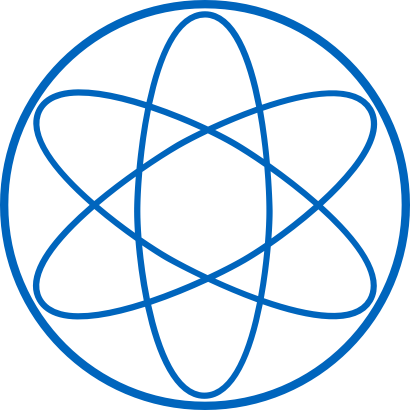
\includegraphics[width=0.2\textwidth]{assets/Physics.png}
        \end{figure}
        \todo{Insert Department Logo}
        \begin{figure}[h]
            \centering
            
\includegraphics[width=0.2\textwidth]{assets/TUM.png}
        \end{figure}
        
    \end{center}
\end{titlepage}

%% page for acknowledgements
\newpage
\section*{Acknowledgments}
\lipsum[1]
\todo[]{add acknowledgements}

\newpage
\section*{Abstract}
\lipsum[2]
\todo{Insert Abstract here}


\newpage
\tableofcontents
\listoftodos\todo{remove todo list when doc is complete}

%% Add lline \input{chapters/chaptername.tex} to add chapter to the tex file%%
\chapter{Introduction}

Tensor Networks in the context of Quantum Error Correction have been used in two distinct places:
\begin{enumerate}
    \item Approximate decoding of QEC Codes
    \item Code construction that come with a natural tensor network decoder
\end{enumerate}



\section{Mathematical Preliminaries}
\subsection{Group Theoretic concepts}
\begin{boxed-defn}{Abelian and Non-Abelian Group}{abelian-group}
A group \(G\) is said to Abelian, iff all the elements of the group pairwise commute with each other under the group operation. It is said to be non Abelian otherwise.\\
\textbf{Examples}
\begin{enumerate}
    \item The group of integers \(\mathbb{Z}\) is Abelian under the addition operation.
    \item The set of \(2 \times 2\) matrices under matrix multiplication form a non-Abelian group.
\end{enumerate}
\end{boxed-defn}

\subsubsection{Pauli Group}
The Pauli matrices \(I, X, Y,Z\) form a group. The \(n\)-qubit Pauli group is defined as follows
\begin{boxed-defn}{n-Qubit Pauli group}{pauli-group}
\begin{equation}\label{eqn: pauli-group}
    \mathcal{G}_n = \{f: f = c\sigma_1 \otimes \sigma_2 \otimes \dots \otimes \sigma_n\} \quad \text{where} \quad \sigma_j \in \{I, X, Y, Z\} \ \text{and} \ c \in \{\pm 1, \pm i\}
\end{equation}
\end{boxed-defn}
Equivalenty single qubit Pauli operators are also defined on a index notation with the following definition
\begin{equation}\label{eqn: pauli-int-map}
    \sigma^0 = I \quad \sigma^1 = X \quad \sigma^2 = Y \quad \sigma^3 = Z
\end{equation}

\subsubsection{Stabilizer Group}

\subsubsection{Coset}

\subsubsection{Lagrange's Theorem}
This is for partitioning the stabilizer group in the disjoint subsets


\section{Stabilizer Quantum Error Correction}
\subsection{Stabilizer Codes}
We consider stabilizer quantum error correcting codes, where the codespace is determined as the subspace of the states which are simultaneously the \(+1\) eigenstates of the stabilizers. The stabilizers are a subset of the \(n\)-qubit Pauli group, \(\mathcal{G}_n\), i.e; \(\mathcal{S} \subset \mathcal{P}_n\). The codespace \(mathcal{H}_0\) can be expressed mathematically as follows
\begin{equation}\label{eqn: codespace}
    \mathcal{H}_0  = {\psi : S \ket{\psi} = \ket{\psi} \forall S \in \mathcal{S}}
\end{equation}
Consider the set of \(r\) independent generators of \(\mathcal{S}\), then \(dim(\mathcal{H}_0) = 2^(n-r)\), where \(n\) is the number of physical qubits. In other words, the number of logical qubits is \(k = n-r\).


\begin{boxed-defn}{Logical Operators of a Stabilizer Code}{stab-log-op}
The logical operators \(\mathcal{L} \subset \mathcal{G}_n\) form a non-Abelian. Given a stabilizer code \(\mathcal{S}\), it's logical operators must obey the following
\begin{enumerate}
    \item It has two sets of generators, X-type and Z-type generators, denoted as \(Z_\alpha, X_\alpha\), with \(\alpha = 1, \dots, k\)
    \item For any \(L \in \mathcal{L}\) and \(S \in \mathcal{S}\), \(LS = SL\)
    \item \(X_\alpha Z_\beta = (-1)^{\delta_{\alpha, \beta}} Z_\beta, X_\alpha\)
\end{enumerate}
\end{boxed-defn}

\begin{boxed-defn}{Destabilisers or Pure Errors}{destabs}
Another group of abelian operators \(P \in \mathcal(G)_n\) are called pure errors (or) destabilisers. They are characterized as follows
\begin{enumerate}
    \item It is a set of \(n-k\) operators \(P_i\) and \(P_i^2 = \mathbb{1}\)
    \item \(P_i S_j = (-1)^{\delta_{i,j}} S_j P_i\) for \(S_j \in \mathcal{S}\) and \(P_i \in \mathcal{P}\)
\end{enumerate}
\end{boxed-defn}

The stabilizers, destabilisers and logical operators together form the \(n\)-qubit Pauli group.

\section{Tensor Network}
\subsection{Tensors}

\subsection{MPS}

\subsection{PEPS}


\subsection{Quantum Circuits as Tensors}
\chapter[]{QEC Code Construction}

This chapter will contain details from both Tensor Network Codes and Quantum Legos
\section{Tensor Network description of stabilizer codes}


\subsection{Example: Surface Code}

\subsection{Example: Bacon Shor Code}


\subsection{Example: Concatenated Codes}

\subsection{Simulating the code}

\section{Quantum Lego description of QECC Codes}


\subsection{Example: Surface Code}

\subsection{Example: Bacon Shor Code}


\subsection{Example: Concatenated Codes}

\subsection{Simulating the code}

\section{Tensor Network Decoder}



\chapter{Decoding of Quantum Error Correcting Codes}

\section{Formal definition of the decoding problem}

\subsection{BSV definiton of Maximum Likelihood decoders}
In this section we formally define MLD. We consider a quantum memory composed of \(n\) physical qubits. Let \(H= (\mathrm{C}^{2})^{\otimes n}\) be the full \(n\)-qubit Hilbert space and \(\mathcal{P}\) be the group of \(n\)-qubit Pauli operators\ref{defn:pauli-group}.


A quantum code of stabilizer type is defined by an abelian stabilizer group \(\mathcal{G} \subset \mathcal{P}\) such that \(-I \notin \mathcal{G}\). Quantum codewords are \(n\)-qubit states invariant under the action of any element of \(\mathcal{G}\). Such states define a codespace \(\mathcal{H}_0 = \{ \psi in  \mathcal{H}: g \psi = \psi \forall g \in \mathcal{G}\}\). The encoding step amounts to initializing the memory in some (unknown) state\(\rho\) supported on the codespace \(\mathcal{H}_0\). We shall consider a stochastic Pauli noise described bya linear map
\begin{equation*}
    \mathcal{N}(\rho)  = \sum_{f \in \mathcal{P}} \pi (f) f \rho f^{\dag}
\end{equation*}
where \(\pi\) is some normalized probability distribution on the Pauli group \(\mathcal{P}\).
Since the initial state \(\rho\) is supported on the codespace \(\mathcal{H}_0\), one has \(f \rho f^{\dag} = \rho\)for any \(f \in \mathcal{G}\). By the same token, \(f \rho f^{\dag} = h \rho h^{\dag}\)whenever \(f\mathcal{G} = h\mathcal{G}\). Given a Pauli operator \(f \in \mathcal{P}\), a subset \(f\mathcal{G}\equiv \{fg: g \in \mathcal{G}\}\)is called a coset of \(\mathcal{G}\). Clearly, \(\mathcal{P}\) is a disjoint union of cosets \(C^{\alpha} = f^{\alpha} \mathcal{G}\), where \(f^{\alpha}\) is some fixed representative of \(C^{\alpha}\). The above shows that errors in the same coset have the same action on the codespace. Thus,
\begin{equation*}
    \mathcal{N}(\rho)  = \sum_{\alpha} \pi (f^{\alpha}\mathcal{G}) f^{\alpha} \rho {f^{\alpha}}^{\dag}
\end{equation*}
where the sum ranges over all cosets of \(\mathcal{G}\) and
\begin{equation*}
    \pi(f\mathcal{G}) = \sum_{g \in \mathcal{G}} \pi(fg)
\end{equation*}

For simplicity, here we assumed that all coset representatives \(\mathcal{f^{\alpha}}\) are hermitian operators. We shall refer to the quantity \(\pi(f \mathcal{G})\) as a coset probability. At the decoding step one attempts to guess the coset of the stabilizer group that contains the actual error based on a partial information about the error known as a syndrome. More precisely, let \(g^1,g^2,\dots,g^n \in \mathcal{G}\) be some fixed set of generators of \(\mathcal{G}\). Since the generators \(\mathcal{g}^i\) pairwise commute, they can be diagonalized simultaneously.


A configuration  of  eigenvalues \(g^i=\pm 1\)can be described by a syndrome \(s \in \{0,1\}^{m}\) such that \(g^i = (-1)^{s_i} \forall i = 1, dots, m\). Assuming that the generators \(g^i\) are independent, there are \(2^m\) possible syndromes. The full Hilbert  space  can  be  decomposed  into a direct sum of syndrome subspaces
\begin{equation*}
    \mathcal{H} = \bigoplus_{s \in\{0,1\}^{m} }  \mathcal{H}_s
\end{equation*}
where \(\mathcal{H}_s = \{ \psi in \mathcal{H}: g^i \psi = (-1)^{s_i} \psi \forall i\}\). Note that the codespace \(\mathcal{H}_0\) corresponds to the zero syndrome. A Pauli operator \(f \in \mathcal{P}\) is said to have a syndromes iff \(f g^i = (-1)^{s_i} g^i f\)for all \(i = 1, \dots, m\). Equivalently, \(f\) has a syndromes iff \(f \mathcal{H}_0 = \mathcal{H}_s\). For each syndrome \(s\) let us choose some fixed Pauli operator \(f(s)\) with the syndrome \(s\). One can easily check that the set of all Pauli operators with  a  syndromes coincides with the coset \(f(s)\mathcal{C}(\mathcal{G})\), where
\begin{equation*}
    \mathcal{C}(\mathcal{G}) = \{ f \in \mathcal{P}: fg = gf \forall g \in \mathcal{G}\}
\end{equation*}
is a group known as the centralizer of \(\mathcal{G}\). Note that \(\mathcal{G} \subseteq \mathcal{C}(\mathcal{G})\). Thus each coset of \(\mathcal{C}(\mathcal{G})\) can be partitioned into a disjoint union of several cosets of \(\mathcal{G}\). Here we only consider stabilizer codes with a single logical  qubit. Let \(X, Y, Z \in \mathcal{C}(\mathcal{G}) \ \mathcal{G} \) the logical Pauli operators on the encoded qubit. Then each coset of \(\mathcal{C}(\mathcal{G})\) consists of four disjoint cosets of \(\mathcal{G}\), namely,
\begin{equation*}
    f(s) \mathcal{C}(\mathcal{G}) = C_{I}^{s} \cup C_{X}^{s} \cup C_{Y}^{s} \cup C_{Z}^{s}
\end{equation*}
where,
\begin{eqnarray*}
    C_{I}^{s} = f(s)\mathcal{G}, \quad C_{X}^{s} = f(s)\bar{X} \mathcal{G} \\
    C_{Y}^{s} = f(s)\bar{Y}\mathcal{G}, \quad C_{Z}^{s} = f(s)\bar{Z} \mathcal{G}
\end{eqnarray*}

The decoding step starts by a syndrome measurement that projects the corrupted state \(\mathcal{N}(\rho)\) onto one of the syndrome subspaces \(\mathcal{H_s}\). The above arguments show that\(f \rho f^{\dag}\) has  support  on \(\mathcal{H}_s\) iff \(f \in f(s)\mathcal{C}(\mathcal{G})\). Thus  the syndrome  measurement  reveals  the  coset  of \(\mathcal{C}(\mathcal{G})\) that contains the  error f,whereas  our  goal  is  to  determine which coset of \(\mathcal{G}\) contains \(f\). Using the above equations, one can write the post-measurement (unnormalized) state as
\begin{eqnarray*}
    \rho(s) = \pi(C_{I}^{s}) . f(s)\rho f(s)           \\
    + \pi(C_{X}^{s}) . f(s)\bar{X}\rho\bar{X} f(s) \\
    + \pi(C_{Y}^{s}) . f(s)\bar{Y}\rho\bar{Y} f(s) \\
    + \pi(C_{Z}^{s}) . f(s)\bar{Z}\rho\bar{Z} f(s) \\
\end{eqnarray*}
where \(s\) is the observed syndrome. Here we assumed for simplicity that \(f(s)\) and the logical operators ̄\(\bar{X}, \bar{Y}, \bar{Z}\)are hermitian. This shows that the effective noise model conditioned on the syndrome can be described by applying one of the four Pauli errors \(f(s), f(s)\bar{X}, f(s)\bar{Y}, f(s)\bar{Z}\) with probabilities \(\pi(C_I^{s}), \pi(C_X^{s}), \pi(C_Y^{s}), \pi(C_Z^{s})\)respectively. Clearly, the best possible error correction algorithm  for  this  effective  noise  model  is  to  choose  a recovery  operator  as  the  most  likely  of  the  four  errors.Equivalently,  we  should  choose  a  recovery  operator  as any Pauli operator that belongs to the most likely of the four cosets \(C_{I}^{s}, C_{X}^{s}, C_{Y}^{s}, C_{Z}^{s}\)which we denoteCsML.  These steps can be summarized as follows.

\begin{boxed-algo}{ML-Decoder}{mld-depolarizing}
\textbf{Input}: syndrome \(s \in \{0,1\}^m\) \\
\textbf{Output}: recovery operator \(g \in \mathcal{P}\) \\

\(f(s) \leftarrow\) any Pauli operator with a syndrome \(s\) \\
\(C_{ML}^{s} \leftarrow\) arg \(max_{\mathcal{C}}\) \(\pi(\mathcal{C})\), where \(\mathcal{C} \in \{C_{I}^{s}, C_{X}^{s}, C_{Y}^{s}, C_{Z}^{s}\}\)
\end{boxed-algo}

The  final  step  of  the  decoding  is  to  apply  the  optimal recovery  operator \(g\).It results in a state \(g \rho(s) g^{\dag}\).We conclude that MLD correctly identifies the coset of \(\mathcal{G}\) that contains the actual error and maps the corrupted state \(\mathcal{N}(\rho)\) back to the encoded state \(\rho\) with a probability
\begin{equation*}
    P_{success} = \sum_{s \in \{0,1\}^{m}} \pi(\mathcal{C}_{ML}^{s})
\end{equation*}
In what follows we shall always ignore overall phase factors of Pauli operators.  Such phase factors are irrelevant for our purposes since they do not change the outcome of error correction.



\subsection{Exact decoding definition of Poulin}
Here we provide more detail on how to compute the logical channel for a round of error correction. Note that, via the Choi-Jamiolkowski isomorphism, a qubit channel \(\mathcal{E}\) is completely described by the \(4 \times 4\) process matrix
\begin{equation*}
    C_{ij} = Tr([P_i \otimes P_j][(\mathcal{E} \otimes \mathcal{I})(\ketbra{\Psi^{+}}{\Psi^{+}})])
\end{equation*}
where \(P_i\) for \(i = 0;1;2;3\) are the identity and Pauli \(X, Y, Z\) matrices respectively. This represents the state obtained when the channel is applied to the first qubit of a Bell state \(\ket{\Psi^{+}} = \ket{00} + \ket{11}\), when expressed in the Pauli basis. Here we will show how to compute \(C_ij\) for the logical channel in the case of surface-code error correction, which will depend on the noise map, the syndrome and the decoder. The simulated error correction process can be decomposed into three parts
\begin{equation*}
    \mathcal{E} = \mathcal{D}_s \circ \mathcal{R}_s \circ \mathcal{N}
\end{equation*}
where \(\mathcal{N}\) is the physical noise map acting on the \(N\) qubits of the code, \(\mathcal{R}_s\) is the recovery map and \(\mathcal{D}_s\) is the decoder correction. The recovery map returns the noisy state to the code space (without performing any classical processing of the syndrome) and can further be decomposed into
\begin{equation*}
    \mathcal{R}_s = T_s \Pi_s \rho \Pi_s T_s
\end{equation*}
where \(\Pi_s\)is a projector onto the subspace corresponding to the syndrome \(s\) and \(T_s\) is a Pauli operator which returns a state in the image of \(\Pi_s\)to the codespace. We have de nedTsas a product of Paulis that connects the flipped \(X\) checks to the top boundary and  flipped \(Z\) checks to the left boundary. The decoder correction \(\mathcal{D}_s\) is the correction selected from \(\{\bar{I}, \bar{X}, \bar{Y}, \bar{Z}\}\) by the decoding algorithm to minimise the logical error.

For now, assume that the decoder does nothing so that \(\mathcal{E} =\mathcal{R}_s \circ \mathcal{N}\). The logical channel \(\mathcal{E}\) is a map from the codespace to itself, so it is effectively a single-qubit map. The process matrix describing the transformation of the logical information given the syndromes is thus
\begin{equation*}
    C_{ij} = Tr([P_i \otimes P_j][( (\mathcal{R}_s \circ \mathcal{N}) \otimes \mathcal{I})(\ketbra{\Psi^{+}}{\Psi^{+}})])
\end{equation*}
where \(\ket{\Psi^{+}}\)is a Bell state of the form \(\ket{\Psi{+} = \ket{0}_L \ket{0}_a + \ket{1}_L \ket{1}_l}\), where the first qubit is encoded into the surface code and the second qubit is an unencoded ancilla qubit that is assumed to be noise free. Using the cyclic property of the trace and the fact that \(T_s \Pi_S = \Pi_0 T_s\), where \(\Pi_0\) is the projection onto the code space, we can write the above expression more explicitly as

\begin{equation*}
    C_{ij} = Tr([T_s P_i T_s \Pi_s \otimes P_j][(  \mathcal{N} \otimes \mathcal{I})(\ketbra{\Psi^{+}}{\Psi^{+}})])
\end{equation*}
In the main text we have shown how to represent the Bell state as a tensor network, and how this tensor-network description changes as local noise \(\mathcal{N}\), and syndrome projectors \(\Pi_s\) are applied to the state. Using this, the trace over the physical indices only

\begin{equation*}
    A_i =  Tr_L([T_s P_i T_s \Pi_s \otimes P_j][(  \mathcal{N} \otimes \mathcal{I})(\ketbra{\Psi^{+}}{\Psi^{+}})])
\end{equation*}
can be represented as a square lattice tensor network, as in 1(d), and can be contracted using the method described in the text. Here \(Tr_L\) indicates that the trace is taken over the physical indices of the logical qubit of \(\ket{\Psi^{+}}\)and the ancilla qubit is left uncontracted, and untouched by the other operators in the trace. Therefore the expression above has two uncontracted indices (the ancilla indices), i.e. it is a \(2 \times 2\) matrix. We use these free indices to compute the target quantities \(C_ij\) via \(C_ij = Tr(P_j A_i)\). Computing \(C_ij\) in this way would seem to require computing four full square lattice tensor contractions: one for each \(A_i\), i.e. each row of \(C_ij\). Having computed the effective logical channel \(\mathcal{R}_s \circ \mathcal{N}\), a decoder correction \(\mathcal{D}_s\) can be incorporated simply by composing the logical channel with the chosen Pauli operator. Here we have shown how to compute the logical channel for a given syndrome and noise model. In the following section we will describe a decoding algorithm based on the above calculations.
% However, as explained in Sec.IIIa lot of the intermediate contractions can be reused for differenti, allowing the full matrixCijto be computed using only two full lattice contractions. The overall complexityof this calculation isO(LW4W) if performed exactly, orO(LW ) using the approximate algorithm.

\subsection*{Exact Decoding}
In the previous section we showed how to compute the logical channel \(\mathcal{E}\) for a given noise model and syndrome. This same calculation allows us to perform exact decoding i.e. to select a optimal correction for a given syndrome. Assume that we are given a syndrome \(s\) and a noise model \(\mathcal{N}\). We can compute \(\mathcal{R_s} \circ \mathcal{N}\) using the method described above. Then computing the optimal correction simply amounts to choosing the \(\mathcal{D}_s\) from \(\{I; X; Y; Z\}\) that minimises the distance of the effective channel from the identity
\begin{equation*}
    d(\mathcal{D}_s \circ \mathcal{R}_s \circ \mathcal{N}, I)
\end{equation*}
where \(d\) can be any distance between operators e.g. diamond distance,  delity, or 2-norm distance. The 2-norm distance is usually used due to its easy computability. If \(\mathcal{R}_s \circ \mathcal{N}\) is calculated exactly, this decoding algorithm is optimal, in the sense that it exactly chooses the correction that minimises the distance of the logical channel from the identity. It involves the exact calculation of \(\mathcal{R}_s \circ \mathcal{N}\) and is therefore exponential, as described above. However, if \(\mathcal{R}_s \circ \mathcal{N}\) is already calculated, the remaining calculations involve manipulations of small matrices and take constant time. Thus choosing an optimal correction requires negligible extra work compared to exactly simulating error correction, and therefore we have used this above optimal decoding in all of our exact simulations. When the approximate contraction algorithm is used, the decoder functions almost identically, except that it uses an approximation of \(\mathcal{R}_s \circ \mathcal{N}\), rather than the exact channel. In this case, due to possible errors in the approximation, the decoding is not guaranteed to be optimal. However it would be interesting to see whether such a decoding algorithm is sufficiently accurate for practical purposes.

\section{Tensor Network Construction of the decoding problem in Quantum Error Correction}



\subsection{MPS construction: BSV}

Let \(f \mathcal{G}\) be one of the cosets \(\{C_{I}^{s}, C_{X}^{s}, C_{Y}^{s}, C_{Z}^{s}\}\) defined earlier. Our goal is to compute the coset probability \(\pi(f\mathcal{G})\). Let \(\pi_1\) be any  probability distribution on the single-qubit Pauli group. For example, \(\pi_1(X) = \pi_1(Y) = \pi_1(Z) = \frac{\epsilon}{3}\) and \(\pi_1(I) = 1 - \epsilon\) for the depolarizing noise with a rate \(\epsilon\). By definition,
\begin{equation*}
    \pi(f\mathcal{G}) = \sum_{g \in \mathcal{G}} \prod_{e} \pi_1 (f_e g_e),
\end{equation*}
where  the  product  ranges  over  all  edges  of  the  surface code lattice. Let us parameterize \(g \in \mathcal{G}\) by binary variables \(\alpha_u, \beta_p \in \{0,1\}\) associated with sites \(u\) and plaquettes \(p\) such that
\begin{equation*}
    g(\alpha ; \beta) = \prod_{u} (A_u)^{\alpha_u} . \prod_{p} (B_p)^{\beta_p}
\end{equation*}
Here we used a convention \((B_p)^0 \equiv I \) and \((A_u)^0 \equiv I \). Let \(e\) be some edge of the surface code lattice with endpoints \(u(e), v(e)\) and adjacent plaquettes \(p(e),q(e)\), see Fig. 5.Let \(g_e\) be the restriction of \(g\) onto the qubit \(e\). Clearly \(g_e\) depends only on the bits \( \alpha_{u(e)}, \alpha_{v(e)}\) and \( \beta_{p(e)}, \beta_{q(e)}\). Thus we can write
\begin{equation*}
    g_e(\alpha; \beta) = g_e( \alpha_{u(e)}, \alpha_{v(e)}; \beta_{p(e)}, \beta_{q(e)} )
\end{equation*}
,where \(g_e(i,j;k,l)\) is a function of just four binary variables \(i,j,k,l \in \{0,1\}\). For  horizontal  edges  located  at the left or the right boundary of the lattice the variable \(\alpha_{u(e)}\) or \(\alpha_{v(e)}\) respectively is missing. Likewise, for horizontal edges located at the top or the bottom boundary the variable \(\beta_{p(e)}\) or \(\beta_{q(e)}\) respectively is missing. We arrive at
\begin{equation*}
    \pi(f\mathcal{G}) = \sum_{\alpha} \sum_{\beta} T(\alpha; \beta)
\end{equation*}
where the sums range over binary strings \(\alpha, \beta \in \{0,1\}^{d(d-1)}\) corresponding to all possible configurations of variables \(\alpha_u, \beta_p\) and

\begin{equation*}
    T(\alpha; \beta) = \prod_{e} \pi_1 ( f_e g_e (\alpha_{u(e)}, \alpha_{v(e)}; \beta_{p(e)}, \beta_{q(e)} ))
\end{equation*}

The righthand side of Eq. (35) coincides with the contraction value of a properly defined tensor network on a two-dimensional grid. To define this tensor network, consider the extended surface code lattice shown on Fig. 6. The extended lattice has three types of nodes which we call \(s\)-nodes, \(h\)-nodes, and \(v\)-nodes. Each \(s\)-node represents a location of a stabilizer (either a site stabilizer \(A_u\)or  plaquette  stabilizer \(B_p\))  while \(h\)-nodes  and \(v\)-nodes represent code qubits located on horizontal and vertical edges of the original surface code lattice respectively. We shall refer to edges of the extended lattice as links todistinguish them from edges of the original surface code lattice.
Consider  any  configuration  of  variables \(\alpha, \beta\) and  the corresponding  term \(T(\alpha; \beta)\) from above. For each site stabilizer \(A_u\), let us copy the corresponding variable \(\alpha_u\)to all links incident to the \(s\)-node \(u\). Likewise, for each plaquette stabilizer \(B_p\), let us copy the corresponding variable \(\beta_p\) to all links incident to the \(s\)-node \(p\).  We obtain a labeling of the links by binary variables \(\gamma(\alpha; \beta)\)  with the property that all links incident to any \(s\)-node have the same label. Let us call such a link labeling valid.  By definition,\(T(\alpha; \beta)\) is a product of terms
\begin{equation*}
    T_e(\alpha; \beta) = \pi_1 ( f_e g_e (\alpha_{u(e)}, \alpha_{v(e)}; \beta_{p(e)}, \beta_{q(e)} ))
\end{equation*}
associated with \(h\)-nodes and \(v\)-nodes \(e\) of the extended lattice. Since \(\alpha\) and \(\beta\) are uniquely determined by the link labeling \(\gamma(\alpha; \beta)\), we can also write \(T_e(\alpha; \beta)\) as a function of \(\gamma\), that is, \(T_e(\alpha; \beta) = T_e(\gamma)\). This shows that
\begin{equation*}
    \pi(f\mathcal{G}) = \sum_{ valid \gamma} \prod_{e \in h,v} T_e(\gamma)
\end{equation*}
where the product is over all \(h\)-nodes and \(v\)-nodes and the sum ranges over all valid link labelings. We can now extend the sum in the equation above to all link labelings \(\mathcal{\gamma}\) by adding extra terms \(T_e(\gamma) \in \{0,1\}\) associated with \(s\)-nodes \(e\) such that \(T_e(\gamma) =1\) iff all links incident to \(e\) have the same label and \(T_e(\gamma) = 0\) otherwise. We arrive at
\begin{equation*}
    \pi(f\mathcal{G}) = \sum_{\gamma} \prod_{e \in h,v} T_e(\gamma)
\end{equation*}
Now the product ranges over all nodes of the extended lattice and the sum ranges over all link labelings. Furthermore, by construction, each term \(T_e(\gamma)\) depends only on the labels of links incident to the node \(e\).The expression in the righthand side of the above equation is known as a contraction  value  of  the  tensor  network  defined  by  the collection of tensors \(T_e(\gamma)\). Tensor networks are usually represented by diagrams like the one shown on Fig. 6 such that each box on the diagram carries a tensor with several indexes.  Indexes of a tensor are associated with the links emanating from the corresponding box.  Diagrams representing the tensors \(T_e(\gamma)\) are shown on Eqs. (39,40,41). All tensor indexes \(i,j,k,l\) on these diagrams take values \(0,1\). For tensors located at the boundary some of the indexes may be missing.  Note that the order of arguments of \(g_e\) is interchanged in Eqs. (40,41).  This is simply because the qubits located on horizontal edges  (\(h\)-nodes)have site stabilizers on the left and on the right whereasqubits located on vertical edges (\(v\)-nodes) have site stabilizers on the top and on the bottom.


\subsection{PEPS Construction}
We define an \(N\)particle PEPS \(\ket{\psi}\) to be a quantum state whose tensor of coefficients \(\psi_{i_1, i_2,\dots,i_N} = \braket{i_1, \dots i_N}{\psi}\) is the contraction of a network  of \(N\)tensors \(\mathcal{T} = \{A_{i_1, \mathbf{\alpha}_1}^{(1)}, A_{i_2, \mathbf{\alpha}_2}^{(2)},\dots, A_{i_N, \mathbf{\alpha}_N}^{(N)} \}\), each of which has one physical index labeled \(i\)and some number of virtual indices labeled \(\alpha\). We assume that the physical particles have dimension \(d\), that each virtual index has bond dimension \(D\),and that the number of virtual indices per tensor in \(\mathcal{T}\)is less than a constant \(n\). This implies that the tensor-network description of \(\ket{\psi}\) is memory efficient: While the tensor \(\psi_{i_1, i_2,\dots,i_N}\) has \(d^N\) entries, each tensor in \(\mathcal{T}\) has at most \(dD^n\) entries, and thus the whole set \(\mathcal{T}\) can be specified with only \(NdD^n\) complex numbers.


We consider the optimized layout of the surface code (add figure), wherem qubits are placed on the vertices of a \(W \times L\) rectangular lattice, and \(x\)-check operators \(A_f = \prod_{i \in f }X_i\)and \(z\)-check operators \(B_f = \prod_{i \in f}Z_i\) are defined on alternating faces of the lattice in a checkerboard pattern. This layout is illustrated in (add figure). The logical qubit state \(\ket{0}_L\) is defined to be the simultaneous \(+1\) eigenspace of all check operators and of the logical operator ̄\(\bar{Z}\), where ̄\(\bar{Z}\) is a string of \(Z's\) along the left boundary of the code. Likewise, the state \(\ket{1}_L\) is fixed by all check operators but is a \(-1\) eigenstate of ̄\(\bar{Z}\);it can be obtained as ̄\(\bar{X}\ket{0}_L\), where ̄\(\bar{X}\) is a product of \(X\) operators along the bottom boundary of the code. Given that the product state \(\ket{0}^{\otimes N}\) has nonzero overlap with \(\ket{0}_L\), and that \(\ket{0}^{\otimes N}\) is a \(+1\) eigenstate of every \(B_f\)and ̄\(\bar{Z}\),we have
\begin{equation*}
    \ket{0}_L \propto \prod_{f} \frac{1}{2} (I + A_f) \ket{0}^{\otimes N}
\end{equation*}
where \(\frac{1}{2}(I+A_f)\) is the projector onto the \(+1\) eigenspace of \(A_f\) and the product is taken over all \(x\)-checks

Let \(W_{i, i^{'},\mathbf{0}}(C)\) be a tensor with two physical indices \(i, i^{'}\) and an arbitrary number of virtual indices \(\mathbf{\alpha} = \alpha_1, \alpha_2,\dots,\) which depends on a \(2 \times 2\) matrix \(C\). Each index of \(W(C)\) has bond dimension two, and the only nonzero entries of \(W(C)\) are
\begin{equation*}
    W_{i, i^{'},\mathbf{0}}(C) = \delta_{i, i^{'}} \quad \text{and} \quad  W_{i, i^{'},\mathbf{1}}(C) = C_{i, i^{'}}
\end{equation*}
where 0(1) means that all virtual indices are set to 0(1), and the symbol \(\delta_{i, i^{'}}\) denotes the Kronecker delta. For convenience, we define \(Q^{\pm} = W(\pm X)\) and \(R^{\pm} = W(\pm Z)\).

Consider the projector \(\frac{1}{2}(I+A_f)\) acting on particles 1,2,3 and 4 ordered clockwise around a face. It can easily be verified that the tensor  \(\bra{i_1, i_2, i_3, i_4} I + A_f \ket{i_1^{'}, i_2^{'}, i_3^{'}, i_4^{'}}\) can be expressed a contraction of four tensors,
\begin{equation*}
    \sum_{\alpha_1, \alpha_2, \alpha_3} Q^{+}_{i_1, i_1^{'},\alpha_1} Q^{+}_{i_2, i_2^{'},\alpha_1, \alpha_2} Q^{+}_{i_3, i_3^{'},\alpha_2, \alpha_3} Q^{+}_{i_4, i_4^{'},\alpha_3}
\end{equation*}
We remark that the tensor description for the projection onto the \(-1\) eigenspace of \(A_f\) is identical to Eq.(3) but with any one of the \(Q^{+}\) tensors replaced with \(Q^-\). Projections onto eigenspaces of \(B_f\) operators can be defined analogously by replacing all \(Q's\) with \(R's\). The tensor network corresponding to the product of projectors in Eq.(1) isobtained by overlapping the tensor projector in Eq.(3) overthe whole lattice.

The state \(\ket{0}_L\) is then obtained by applying this projector to the state \(\ket{0}^{\otimes N}\), which, in the tensor-network picture, corresponds to fixing the second index to zero, thus effectively removing it. A square-lattice tensor network \(\mathcal{T} = \{A_{i_1, \mathbf{\alpha}_1}^{(1)}, A_{i_2, \mathbf{\alpha}_2}^{(2)},\dots, A_{i_N, \mathbf{\alpha}_N}^{(N)} \}\) for the state \(\ket{0}_L\) is thusformed from contractions of \(Q^+\) tensors.
While this tensor network describes the logical \(\ket{0}_L\) state, we need to be able to represent other states in orderto fully characterize the transformation of the encoded information during error correction. Specifically, we want to compute the logical channel \(\mathcal{E}_L\) that is applied to the logical qubit during a round of error correction. By the Choi-Jamiolkowski isomorphism, this channel can be inferred directly from the resulting output when a Bell state of the form \(\ket{\Psi{+} = \ket{0}_L \ket{0}_a + \ket{1}_L \ket{1}_l}\) input, where the first qubit is encoded in a surface code and is subject to error correction, while the second qubit i sunencoded and assumed to be noise free. We can obtaina tensor-network description for \(\ket{\Psi^+}\) by a simple modification to the tensor network describing \(\ket{0}_L\). Consider the tensor
\begin{equation*}
    \bar{CNOT} = \sum_{\alpha_1, \alpha_2, \alpha_3} Q^{+}_{i_1, i_1^{'},\alpha_1} Q^{+}_{i_2, i_2^{'},\alpha_1, \alpha_2}  \dots Q^{+}_{i_4, i_4^{'},\alpha_L, \alpha_a}
\end{equation*}
which can be thought of as an \(L\) qubit operator (expressed in tensor form) with a single uncontracted virtual index \(\alpha_a\), which we call the ancilla index. If \(\alpha_a\) is set to 0, then \(\bar{CNOT}\) is simply the identity on its physical indices, while if \(\alpha_a =1\), \(\bar{CNOT}\) is an \(L\)-fold tensor product of \(X\). Therefore,if \(\bar{CNOT}\) is applied to the bottom row of the tensor network for \(\ket{0}_L\), the resulting tensor-network state \(\psi_{i_1, i_2,\dots,i_N, \alpha_a} = \braket{i_1, i_2,\dots,i_N, \alpha_a}{\psi}\) (which includes the ancilla index as a physical particle) will be the desired Bell state \(\ket{\Psi{+} = \ket{0}_L \ket{0}_a + (\bar{X}\ket{0}_L) \ket{1}_l}\)


\subsection{Circuit Construction: Ferris Poulin}
The notes from the Ferris Poulin Paper


\subsection{MLD of concatenated Block codes}
Concatenated Block codes can be constructed using Tensor Networks. This section will have the proof that tensor network contraction decoding is the same as the maximum likelihood decoding.


% \todo{Add references to sections}
% \todo{Add refernces to figures}
% \todo{Make refernce naming nomenclature consistent}

% References%
\newpage
% \newgeometry{top=10mm, bottom=20mm, right=25mm, left=25mm}
\addcontentsline{toc}{chapter}{References}
\nocite{*}
\printbibliography[title=\refname]

\restoregeometry
\newpage

\section*{Appendix}
\addcontentsline{toc}{chapter}{Appendix}
\lipsum[1]




\end{document}